%
%  $Description: Author guidelines and sample document in LaTeX 2.09$ 
%
%  $Author: Jaykumar Patel, Afnan Mir, Nidhi Dubagunta $
%  $Date: 2024/01/28 15:20:59 $
%  $Revision: 1 $
%

% \documentclass[times, 10pt,twocolumn]{acmart} 
\documentclass[times, 10pt,twocolumn]{article} 
\usepackage{latex8}
\usepackage{times}
\usepackage{graphicx}
\usepackage{subcaption}
\usepackage{algorithm}
\usepackage{algorithmic}
\usepackage{adjustbox}
\usepackage{enumitem}
\usepackage{float}

%------------------------------------------------------------------------- 
% take the % away on next line to produce the final camera-ready version 
% \pagestyle{empty}

%------------------------------------------------------------------------- 

\begin{document}

\title{Carbon Aware Serverless System - Group 6}

\author{Jaykumar Patel\\
% The University of Texas at Austin\\
patel.jay4802@utexas.edu\\
jnp2369\\
\and
Afnan Mir\\
% The University of Texas at Austin\\
afnanmir@utexas.edu\\
amm23523\\
\and
Nidhi Dubagunta\\
% The University of Texas at Austin\\
nidhi.dubagunta@utexas.edu \\
nsd632\\
}



\maketitle
\thispagestyle{empty}

\begin{abstract}
   % Serverless computing enables developers to build and deploy applications faster without having to worry about provisioning resources and managing infrastructure. Existing serverless computing systems utilize policies that govern how resources, such as the number of vCPUs and memory, are allocated for a function invocation, but these policies do not consider the carbon footprint of the resources. Furthermore, existing systems do not utilize dynamic frequency scaling (DFS), which scales the frequency that the vCPUs runs at. We propose introducing the frequency at which vCPUs run as a new resource to allocate per invocation. Our system will manage DFS, along with traditional resource allocation (vCPU) to meet service-level objectives (SLO) while minimizing the carbon footprint. Firstly, we will define how to measure carbon emissions. Then we perform a measurement study, which will involve running a variety of workloads on a variety of resource configurations and acquiring their resource usage, carbon emission, and performance in terms of duration. We also conduct a study to determine the carbon emission over the various stages of a function invocation. This will allow us to understand carbon emission during different stages of a serverless function’s lifecycle, how carbon emission varies with changes in vCPU, how carbon emission varies with different inputs to the same serverless function, and how carbon emission varies with dynamic frequency scaling (DVFS). Then, we will adapt OpenWhisk, an open source and serverless cloud platform, to incorporate Bayesian Optimization to drive a carbon-aware DFS and resource allocation model, where frequency to the vCPU will be considered as a resource along with vCPU. We will use this framework to investigate whether machine learning techniques are effective in driving carbon-aware decisions by evaluating our framework’s carbon emissions against OpenWhisk’s current policies. Further work may include creating a framework for the keep-alive policy and scheduling to further minimize carbon footprint. The ultimate goal of this project is to minimize the carbon footprint while meeting each invocation’s SLOs, which are tailored for the individual workloads and determined by metrics such as latency, throughput, total runtime, resulting cost, etc. Though our system should contribute to environmental sustainability, it must also consistently meet the specified operational criteria essential for their intended functions.
   Serverless computing is a method that enables developers to build and deploy applications without having to provision resources or manage infrastructure. However, existing serverless systems do not consider the carbon footprint of function invocations when allocating or configuring resources, such as memory and vCPU. In this paper, we propose a carbon-aware serverless system that focuses on minimizing the carbon emissions of function invocations while continuing to meet service level objectives (SLOs) by finding an optimal configuration for vCPU count and operational frequency of the vCPU cores. We first perform a measurement study by running a variety of workloads with different resource configurations to understand the relationship between resource usage, energy consumption, and performance. We also collect measurements for energy consumption during different stages in the serverless function invocation lifecycle. Leveraging these insights, we aim to incorporate a Bayesian Optimization algorithm into OpenWhisk, an open-source serverless cloud platform, to build a serverless system that performs carbon-aware dynamic frequency scaling (DFS) and vCPU allocation. 
\end{abstract}


\section{Introduction}
% Reduce the abstract, and move a lot of the detailed information here

% Briefly explain how current serverless function invocations work (lifecycle), and give quick intro about what we will be doing.
The rise of cloud computing has transformed the space of digital infrastructure, offering higher amounts of scalability, flexibility, and cost-effectiveness compared to on-premise solutions. Within cloud computing, the concept of serverless computing emerged, which further increased efficiency in application development by abstracting the complexities of infrastructure management and resource provisioning. 

In a serverless system, when a function is invoked, the system checks for a pre-existing warmed container to host the function. If no warmed container is available, a cold start is initiated, during which the runtime environment is set up, necessary dependencies are installed, and the function code is loaded. After the function is executed, the container can remain idle for a period of time for future invocations before it is killed.

Several existing serverless systems, such as AWS and GCP, couple memory and CPU allocation, assigning a CPU share proportional to the memory requested by the user, or using a preset resource allocation option \cite{bibal2023acm}. Serverless systems today also do not incorporate dynamic frequency scaling (DFS), in which the operating frequency of the vCPU cores can be dynamically modified. These policies used for resource allocation are carbon-agnostic, meaning they do not consider the carbon emissions of the function execution and idle containers.

In this paper, we propose a serverless framework that provisions resources based on workload characteristics to minimize the carbon emissions associated with the function invocation, while continuing to meet SLOs, such as total runtime. We introduce the frequency at which vCPUs run as a new resource to allocate per invocation. Our system will optimize the number of vCPUs allocated, as well as the frequency at which the vCPU cores operate. 

\section{Motivation}
% We can include information about the impact of server centers on carbon emissions, and how vCPU and frequency plays a role.

According to a study by Microsoft and the Green Software Foundation, data centers and data transmission networks account for almost 1\% of energy-related greenhouse gas emissions, which contribute to rising global temperatures and climate change \cite{carbon_aware_computing}. By adopting carbon-aware computing, these data centers can play a significant role in decarbonization efforts. 

% Carbon-aware computing not only places emphasis on minimizing carbon emissions associated with deploying and maintaining cloud infrastructures (or in our case serverless functions), but also on optimizing hardware utilization.       


% Through optimizing the amount of vCPU allocated and the frequency of the cores for each specific function invocation, we can both work to minimize the total energy expenditure and therefore carbon footprint, as well encourage high resource utilization, by catering to the specific performance patterns of the function. 
The boxplot in Figure \ref{fig:energy_boxplot}, 
shows the variability in energy consumption (in joules (J)) for different functions with a fixed input, while changing the amount of vCPUs allocated and the frequency at which the cores run. The large range of energy consumption for the same function due to changes in vCPU count and frequency underscores the importance of understanding the relationship between these factors and energy usage. This motivates further study into optimizing vCPU allocation and frequency at a function-level to minimize energy consumption and therefore carbon footprint. 


\begin{figure}[ht]
   \centering
   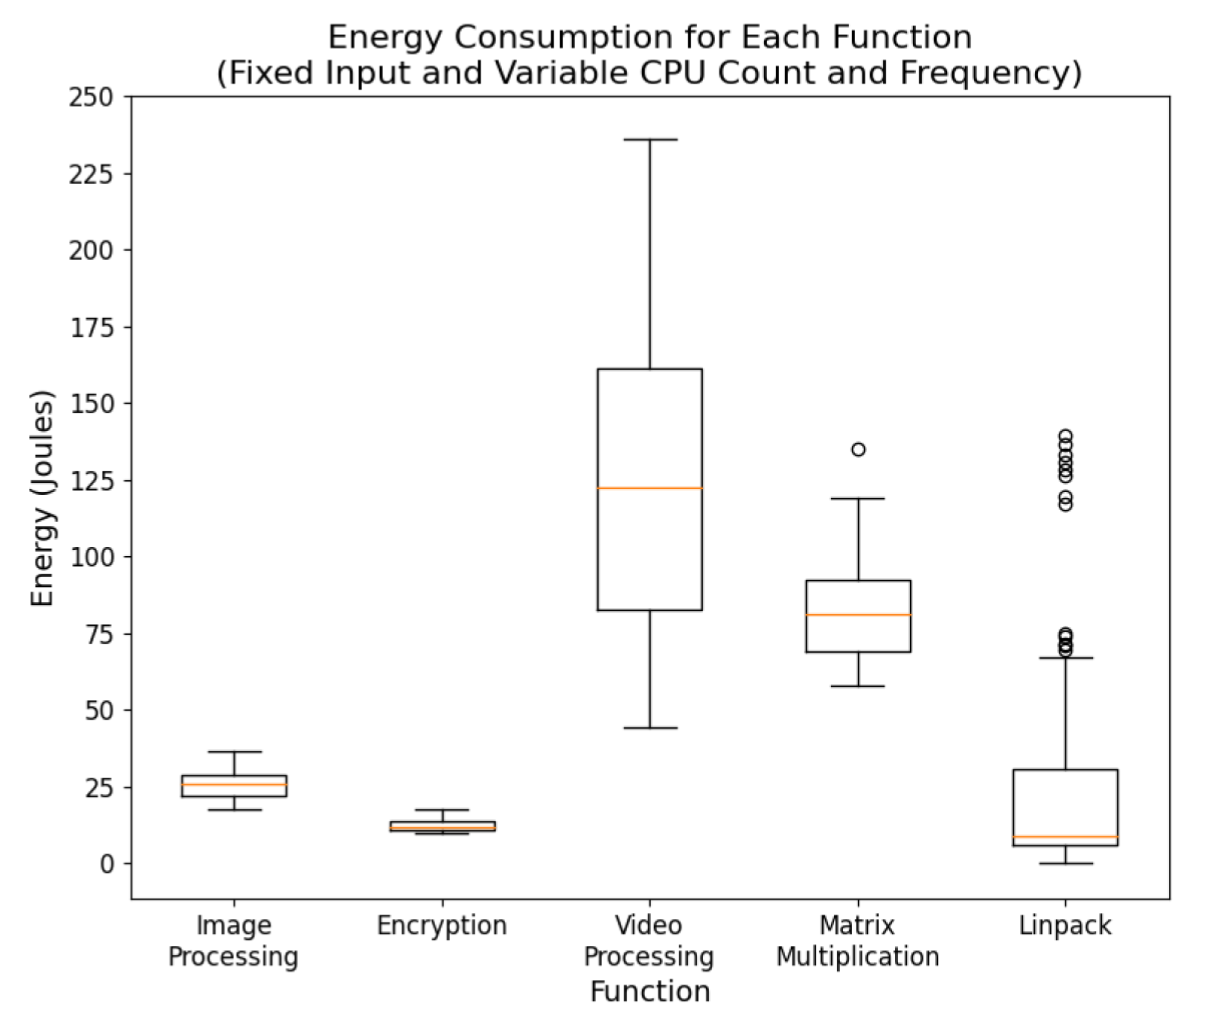
\includegraphics[width=0.45\textwidth]{imgs/energy_boxplot.png}
   \caption{Boxplot showing energy variability across functions with fixed input, while changing vCPU count and frequency. }
   \label{fig:energy_boxplot}
 \end{figure}
\section{Related Work}
% Include CherryPick and Aquatope
CherryPick \cite{CherryPick} is a framework that was developed to find optimal or near-optimal cloud configurations (vCPU and memory) for repetitive big data analytics jobs, addressing challenges of system cost, performance, and adaptivity. CherryPick leverages Bayesian Optimization (BO) to build performance models that are able to determine optimal or near-optimal configurations that satisfy performance constraints with a relatively low number of samples. 

Aquatope \cite{AQUATOPE} also utilizes Bayesian models to optimize for resource allocation for serverless function invocations. This framework also utilizes BO to learn the mapping from resource configuration to performance and cost, while considering noise and uncertainty in the cloud environment. Aquatope also uses batch sampling to reduce the cost of exploration when finding a resource configuration.

Our work aims to draw from the ML techniques utilized in CherryPick and Aquatope. We plan to use BO to find the near-optimal configuration of vCPU and operational frequency with the objective of minimizing carbon footprint for serverless function invocations. We will also set performance constraints to ensure user-specified SLOs are met.

In the space of carbon-aware computing, GreenCourier \cite{GreenCourier} is a scheduling framework that enables runtime scheduling of serverless functions across geographically distributed regions based on their carbon efficiencies. This work focuses on minimizing carbon footprint based on the location at which a function is run, whereas our work aims to optimize the host environment through proper resource allocation and configuration to minimize carbon emissions using function-level characteristics.

\begin{table*}[htbp]
   \centering
   \begin{tabular}{|c|c|}
   \hline
   \textbf{Variable} & \textbf{Values} \\ \hline
   Function Type & Float Matrix Multiplication, Image Processing, Video Processing, Encryption, Linpack \\ \hline
   vCPU Count & 1, 2, 3, 5, 7, 10, 13, 16, 19, 22, 25, 28, 31 \\ \hline
   vCPU Frequency (GHz) & 1.0 to 2.4 in 0.2 increments\\ \hline
   \end{tabular}
   \caption{Measurement Study Configurations -- Energy Variation with vCPU and Frequency Allocation}
   \label{tab:mstudy1_configurations}
\end{table*}

\begin{table*}[htbp]
  \centering
  \begin{tabular}{|c|c|}
  \hline
  \textbf{Variable} & \textbf{Values} \\ \hline
  Image & main-python, video-ow, mobilenet-ow, sentiment-ow, audio-ow \\ \hline
  vCPU Count & 1, 2, 3, 4, 5, 6, 7, 8, 9, 10, 12, 14, 16, 18, 20, 22, 24, 26, 28, 30, 32 \\ \hline
  Memory (MB) & 512 to 10240 in 512 increments\\ \hline
  \end{tabular}
  \caption{Measurement Study Configurations -- Energy Variation with vCPU and Frequency Allocation}
  \label{tab:mstudy1_configurations}
\end{table*}

\section{Measuring Carbon Emission}


Before conducting the measurement study, we need to define how to measure carbon emissions. According to Gupta et al. \cite{gupta2022act}, the carbon footprint of a server can be calculated using the following formula where $OP_{CF}$ is the operational carbon footprint, $CI_{use}$ is the carbon intensity of the energy source, and $Energy$ is the operational energy:

\begin{equation}
   OP_{CF} = CI_{use} \times Energy
\end{equation}

The carbon intensity refers to how \textit{clean} the energy source is. For example, coal has a higher carbon intensity than solar. We assume that the energy source of the serverless system is constant, and therefore, the carbon intensity is constant. We can then use the operational energy as a proxy for the carbon footprint.

\subsection{Measuring Energy}
We first need a way to measure the energy consumption of a serverless function invocation. EnergAt \cite{he2023hotcarbon} is a tool that measures fine-grained energy consumption at the thread-level while taking into account NUMA effects. An EnergAt process continuously samples a target container, where each sample returns energy readings over an interval of at least 50ms. Therefore, EnergAt will get continuous back-to-back samples of energy readings over time. The energy consumption of a target container is the sum of the energy readings over the duration of the function invocation. One limitation of EnergAt is that every target container for which we want to measure energy consumption must be instrumented with its own EnergAt process. This is not feasible as the number of EnergAt processes and resource contention scales with the number of target containers.

To mitigate this issue, we created EnergyLiteDaemon. EnergyLiteDaemon is a daemon that samples multiple target containers in a round-robin fashion, where each sample returns energy readings over an interval of at least 50ms. This allows us to measure the energy consumption of multiple target containers with a single, lightweight, process. Due to the round-robin fashion, however, the sampling frequency per target container decreases as a function of the number of target containers. If there are multiple containers, the samples are no longer back-to-back -- there may be some time delay between two samples. To solve this, we complete the following steps to interpolate the total energy consumption of a target container:

\textbf{Power Calculation:} We compute the average power for every sample by dividing the energy consumed over the interval of the sample by the duration of that interval. This allows us to get a power-time scatter plot that contains $n$ points, where $n$ is the number of samples.

\textbf{Trapezoidal Integration:} Given a power-time scatter-plot, we compute the total energy consumption of a target container using trapezoidal integration. All of the points in the power-time scatter plot are connected by straight lines, and the area under the curve is calculated. This area is the total energy consumption of the target container. 

A toy example of energy measurement using EnergAt and EnergyLiteDaemon is shown in Appendix \ref{appendix:energy_measurement}.

Due to EnergyLiteDaemon's round-robin sampling approach, which reduces its overhead, it may not capture all energy readings for a container. Even with trapezoidal integration, the energy consumption will not be exact. To determine the accuracy of EnergyLiteDaemon, we ran 20 stress docker containers, with varying CPU usage and duration. Figure \ref{fig:EnergyLiteDaemon_Efficacy} shows the energy consumption of the containers as measured by EnergAt and EnergyLiteDaemon. The absolute percentage error of EnergyLiteDaemon is less than 15\%, which is acceptable for our purposes.

\begin{figure}[ht]
   \centering
   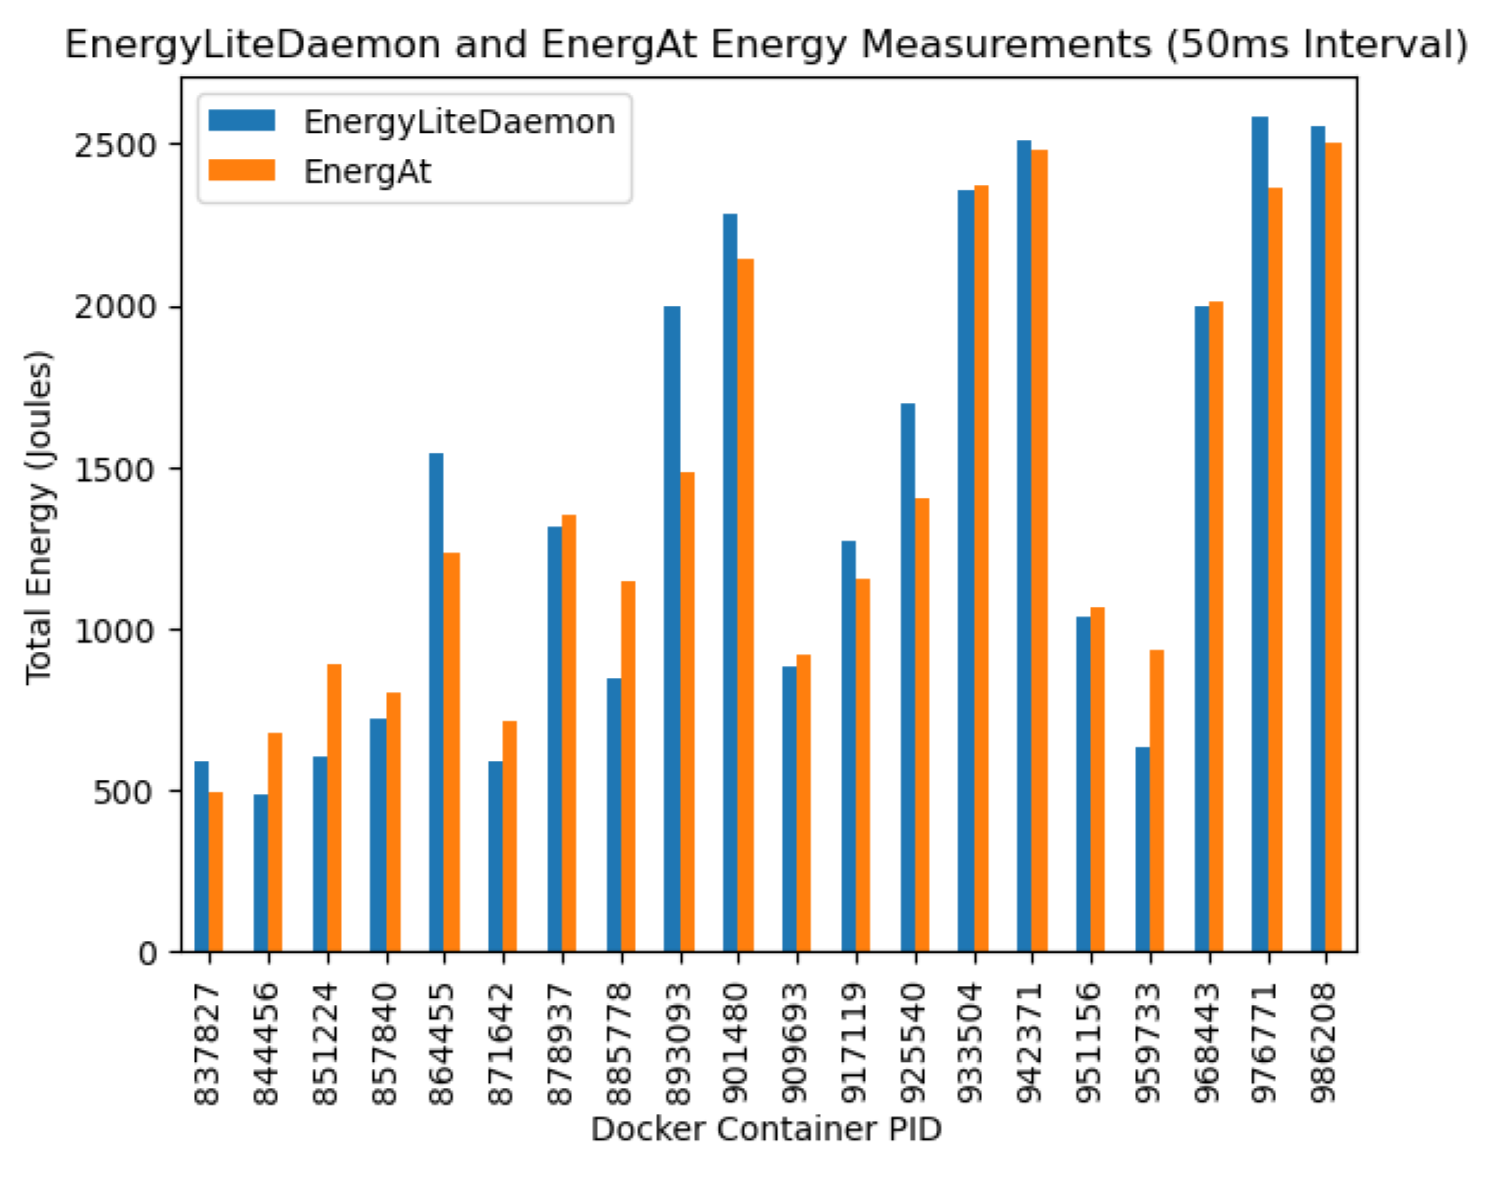
\includegraphics[width=0.45\textwidth]{imgs/EnergyLiteDaemon_Efficacy.png}
   \caption{Energy measurements of EnergAt and EnergyLiteDaemon for 20 stress docker containers.}
   \label{fig:EnergyLiteDaemon_Efficacy}
 \end{figure}

\section{Measurment Study}

We conduct two measurement studies to answer the following questions: \textbf{1. How does energy vary with changes in vCPU and frequency allocation? 2. What is the energy consumption over the lifecycle of a serverless function invocation?}

To perform the measurement study, we use OpenWhisk, which is an open-source serverless platform, to run function invocations. We use EnergyLiteDaemon to measure the energy consumption of the function invocations.

\subsection{Energy Variation with vCPU and Frequency Allocation}

A variety of workloads were run on different vCPU and frequency configurations. We collected the vCPU utilization, energy consumption, and performance in terms of duration. The resource configurations are shown in Table \ref{tab:mstudy1_configurations}.

We then analyzed the data to understand how energy consumption varies with changes in vCPU and frequency allocation. For float matrix multiplication, energy usage initially decreases and then flat-lines as the vCPU allocation increases. This is because matrix multiplication is highly parallelizable and has high vCPU utilization, leading to a decrease in duration and energy usage. For image processing, energy usage has no apparent correlation with vCPU allocation, likely because most of the image processing tasks are non-parallelizable. For encryption, energy usage, duration, and vCPU utilization do not change with vCPU allocation because encryption is also non-parallelizable and does not benefit from additional vCPUs.

For both types of functions, energy consumption as a function of frequency displays a convex curve, where energy consumption decreases with frequency until a certain point (which varies between different functions and function inputs), and then begins to increase again. This is because the energy consumption per time unit of a vCPU is proportional to the frequency at which it runs, but the overall duration of the function is inversely proportional to the frequency at which the vCPU runs. More details on the results can be found in Appendix \ref{appendix:energy_variation_vcpu_frequency}.

These trends support the idea that we can use machine learning to learn the relationship between vCPU, frequency, and energy consumption, and use this model to minimize energy consumption while meeting SLOs.

\subsection{Energy Consumption Over the Lifecycle of a Serverless Function Invocation}
Additionally, we ran a variety of docker images, each of a different size, with a variety of vCPU and memory configurations to investigate carbon emissions of different stages of the container lifecycle. For each (image, vCPU, memory) configuration, we measured the energy consumption at different stages of the function invocation lifecycle. More specifically, we measured the energy consumed during the container spin-up, the idle time, and the container spin-down.

After collecting and analyzing the data, we first found that for each stage of the lifecycle we measured, when changing the vCPU and memory configurations, the energy consumption did not vary significantly. This was true for all image sizes. This is likely due to the fact that these resources will not actually be allocated to the container until the compute inside the container requires them. We did notice that if we varied the image size, the energy consumption of the container spin-up process significantly increased as the image size increased. However, it is worth noting that most of the energy consumption of the spin-up is accredited to the `docker pull' process, which would only be a one-time operation. The `docker run' does not consume a significant amount of energy and does not show any statistical correlation. For the idle time, we noticed a strange negative correlation trend with the image size, and for the spin-down, we noticed a somewhat positive correlation with a few outlier points. Since we only used a few image sizes, we cannot definitively conclude that these trends will extrapolate.

Due to our findings of little to no correlations, we decided to not pursue a carbon-aware keep-alive policy further. More details on the study can be found in Appendix \ref{appendix:energy_variation_vcpu_memory}.

% \section{Tentative System Overview}


% \section{Experimental Setup}


% \section{Results}


\section{Final System}

\subsection{Machine Learning Model}
To implement a machine learning model to minimize carbon emissions, we plan on using BO model similar to \cite{CherryPick} and \cite{AQUATOPE}. We will optimize vCPU allocation and frequency scaling to minimize carbon with meeting SLOs as our constraint. Since we have collected data on 5 different functions, we will have a separate BO model for each function. Each function and its input will be encoded into an input vector for the BO model, either using feature engineering or a neural encoder similar to \cite{AQUATOPE}. Then, the vCPU count and frequency will be concatenated to this input vector, and the BO model will search the space of vCPU count and frequency to minimize energy usage. The output of the BO model will be the vCPU count and frequency that minimizes energy usage while meeting SLOs. A diagram of the machine learning model is shown in Figure \ref{fig:ml_model}.

\begin{figure}[ht]
   \centering
   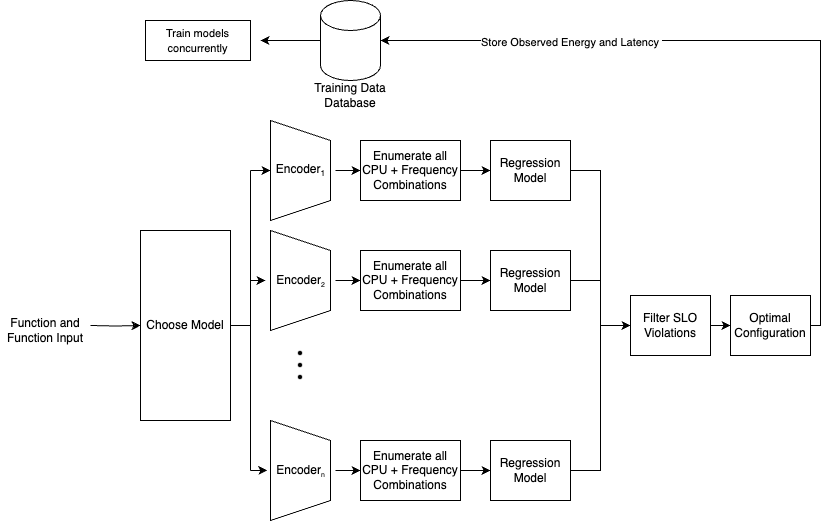
\includegraphics[width=0.45\textwidth]{imgs/ml_model.png}
   \caption{Bayesian Optimization Model for Carbon-Aware Serverless System}
   \label{fig:ml_model}
 \end{figure}
\subsection{Adapting OpenWhisk}

\begin{figure}[ht]
   \centering
   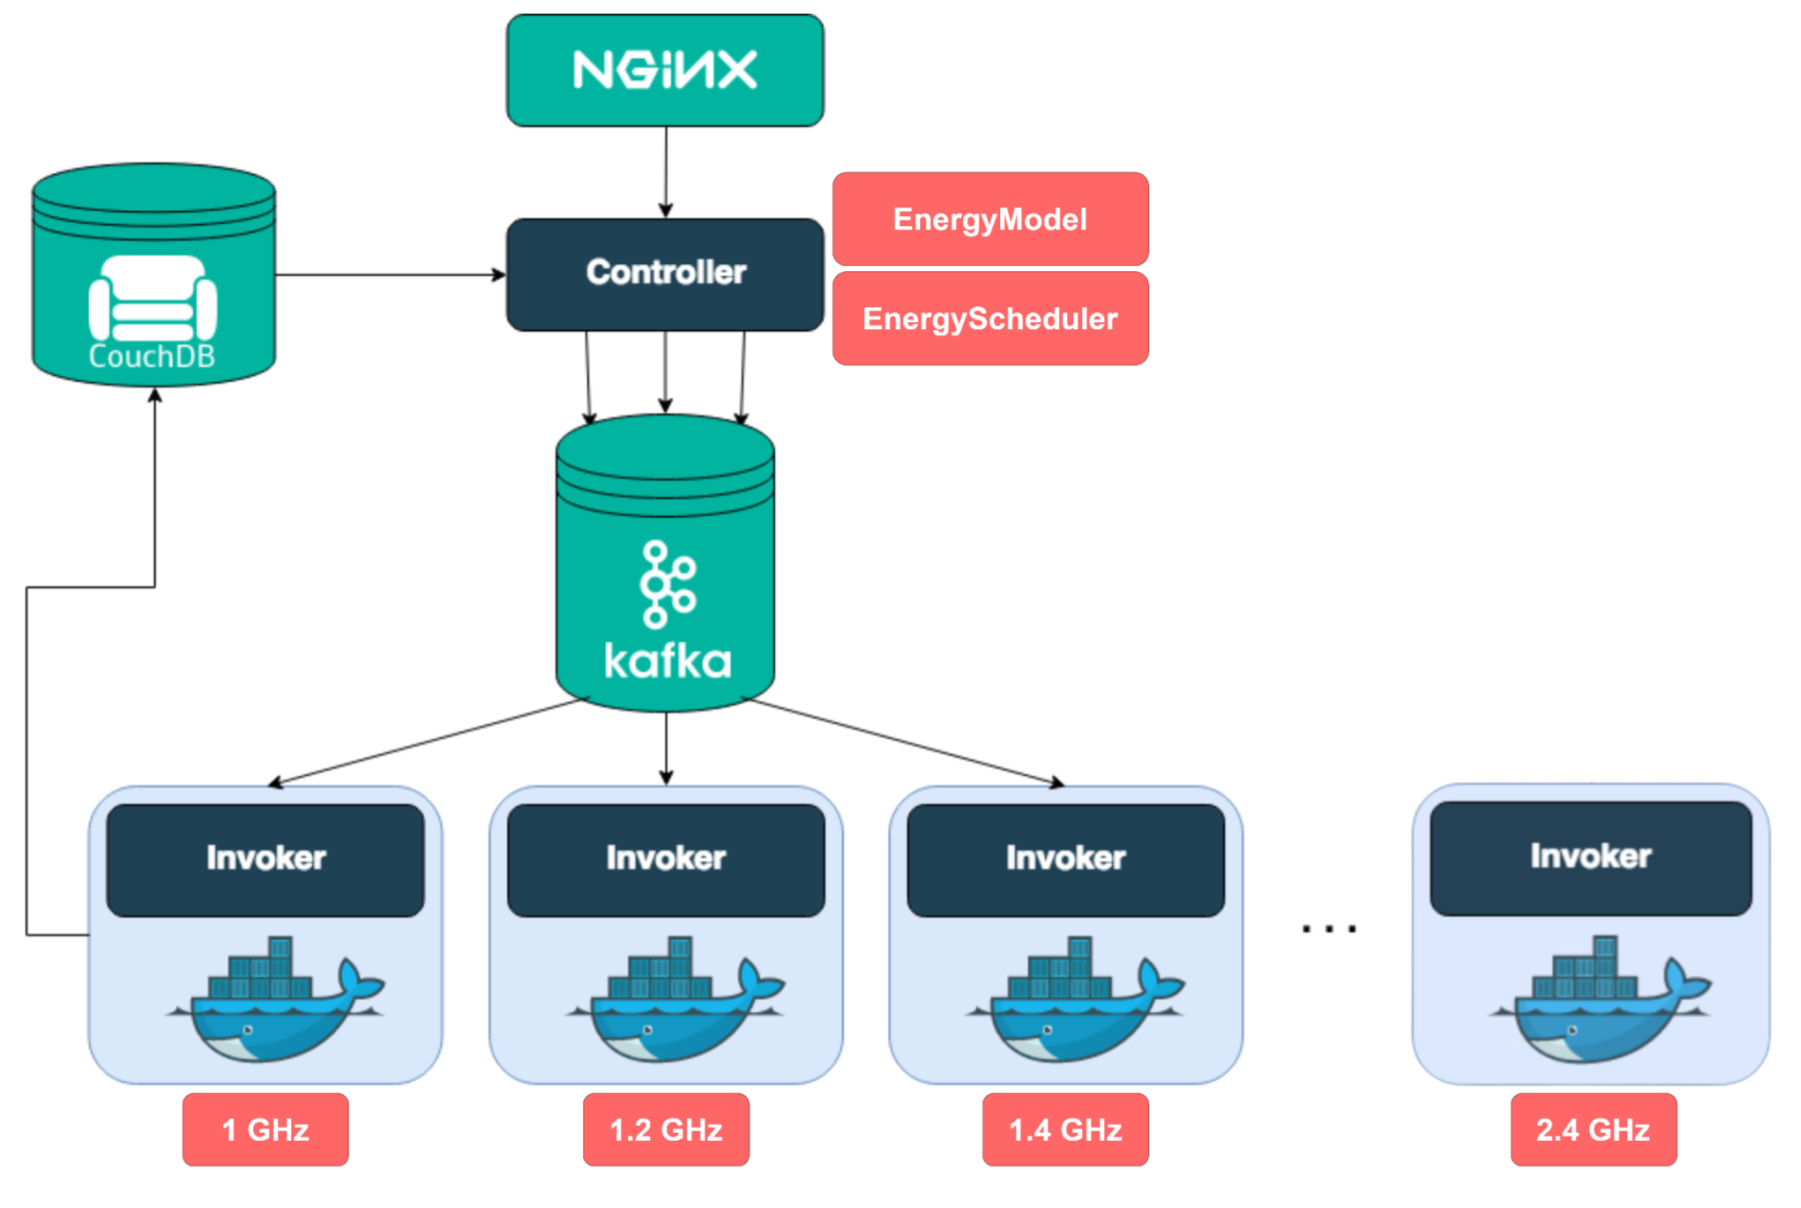
\includegraphics[width=0.45\textwidth]{imgs/Adapted_OW_System_Overview.png}
   \caption{Adapted OpenWhisk System Overview}
   \label{fig:adapted_ow_system_overview}
 \end{figure}

We adapted OpenWhisk to incorporate Bayesian Optimization to drive a carbon-aware DFS and vCPU allocation model. Figure \ref{fig:adapted_ow_system_overview} shows the system overview.

The Bayesian Optimization model is contained in a shim layer, called the EnergyModel. Whenever a user invokes a function, the EnergyModel determines the optimal vCPU and frequency allocation (using Bayesian Optimization). The EnergyModel is trained online periodically at 30 second intervals.

We created a custom scheduler, called EnergyScheduler, that replaces OpenWhisk's current scheduler. There are multiple invoker nodes, each running at a different frequency, as shown in \ref{fig:adapted_ow_system_overview}. The EnergyScheduler uses the output of EnergyModel to determine which invoker to send the function invocation to. We base the EnergyScheduler's algorithm off of Shabri's scheduler \cite{sinha2024shabari}. EnergyScheduler is designed to mitigate cold starts by:

\textbf{1. Prioritizing routing the invocation to warm containers: } The scheduler will receive the invocation and the predicted vCPU and frequency allocation from the EnergyModel. The scheduler will then iterate through the invokers running at at least the predicted frequency and attempt to find a warm container that is closest to the predicted vCPU allocation. If a warm container is found, the invocation is sent to that container. If no warm container is found, the invocation is send to the invoker running at the predicted frequency.

\textbf{2. Premptively spinning up containers: } In the case that the invocation is sent to an invoker running at higher than the predicted frequency or with more vCPUs than predicted, the scheduler will preemptively spin up a container on the invoker running at the predicted frequency with the predicted vCPU allocation. This is done to mitigate future cold starts and underutilization of resources. The underlying assumption is that function invocations exhibit temporal locality, meaning that in a short time frame, the same function is likely to be invoked again. Thus, preemptively spinning up a container will reduce the likelihood of cold starts for future invocations.

\section{Evaluation}

\subsection{Methodology}
\textbf{Workloads.} We evaluate our system using functions shown in Table \ref{tab:summary_of_serverless_functions}. These are the same functions used in the measurement study. These functions vary in their parallelizability and resource requirements, making them suitable for evaluating the effectiveness of our system. We utilize the same trace used in Shabri \cite{sinha2024shabari} to simulate function invocations, which is a scaled down sample of the Azure trace. We utilize a requests per second (RPS) of 1 for the evaluation.

\begin{table*}[htbp]
  \centering
  \begin{tabular}{|c|c|c|c|c|}
  \hline
  \textbf{Function} & \textbf{Input Type} & \textbf{\# Runs} & \textbf{Sizes} & \textbf{Size Range} \\ \hline
  floatmatmult & square matrix & 1 & 1 & 1 \\ \hline
  linpack & square matrix & 1 & 1 & 1 \\ \hline
  encrypt & string & 1 & 1 & 1 \\ \hline
  imageprocess & image & 1 & 1 & 1 \\ \hline
  videoprocess & video & 1 & 1 & 1 \\ \hline
  \end{tabular}
  \caption{Summary of serverless functions studied.}
  \label{tab:summary_of_serverless_functions}
\end{table*}

\textbf{Metrics.}

\textbf{Baselines.} We compare our system to two baselines Parrotfish and Aquatope. Parrotfish \cite{parrotfish} utilizes parametric regression to predict resource configuration, while Aquatope \cite{aquatope} uses Bayesian Optimization to predict resource configuration. Neither of the aforementioned baselines consider optimizing for energy efficiency. Furthermore, the original OpenWhisk's scheduler was used when running Parrotfish and Aquatope. Furthermore, Parrotfish only optimizes memory allocation; thus, we allocate CPU proportional to memory. Since our system only optimizes CPU and frequency, we run our system three times: 1. using Parrotfish's memory predictions, 2. using Aquatope's memory predictions, 3. constant value of 4096 bytes. We compare our system to these baselines in terms of energy consumption and SLO violations.

\subsection{Results using EnergyLiteDaemon}
We ran the experiment for Parrotfish, Aquatope, and our system, where EnergyLiteDaemon was used to collect energy consumption data.

\subsubsection{Energy Comparison}

\subsubsection{SLO Violations Comparison}

\subsection{Results using Energat}

\subsubsection{Energy Comparison}

\subsubsection{SLO Violations Comparison}


\section{Discussion}

\section{Conclusion}

% \section{Conclusion}

\bibliographystyle{latex8}
\bibliography{latex8}

\appendix
\section{Appendix}
\subsection{Energy Measurement}
\label{appendix:energy_measurement}
A toy example of the energy measurement of a container using EnergAt and EnergyLiteDaemon is shown in Figure \ref{fig:energy_toy_example}. Figure \ref{fig:a} shows the energy readings of EnergAt. Figure \ref{fig:b} shows the energy readings of EnergyLiteDaemon. EnergyLiteDaemon doesn't capture all energy readings for the container due to the round-robin sampling approach. Figure \ref{fig:c} shows EnergyLiteDaemon's power calculation of each energy sample. Figure \ref{fig:d} shows the energy interpolation of EnergyLiteDaemon using trapezoidal integration.

\begin{figure*}[ht] % Note the use of figure* instead of figure
   \centering
   \begin{subfigure}[b]{0.24\textwidth} % Adjusted width to fit across two columns
         \centering
         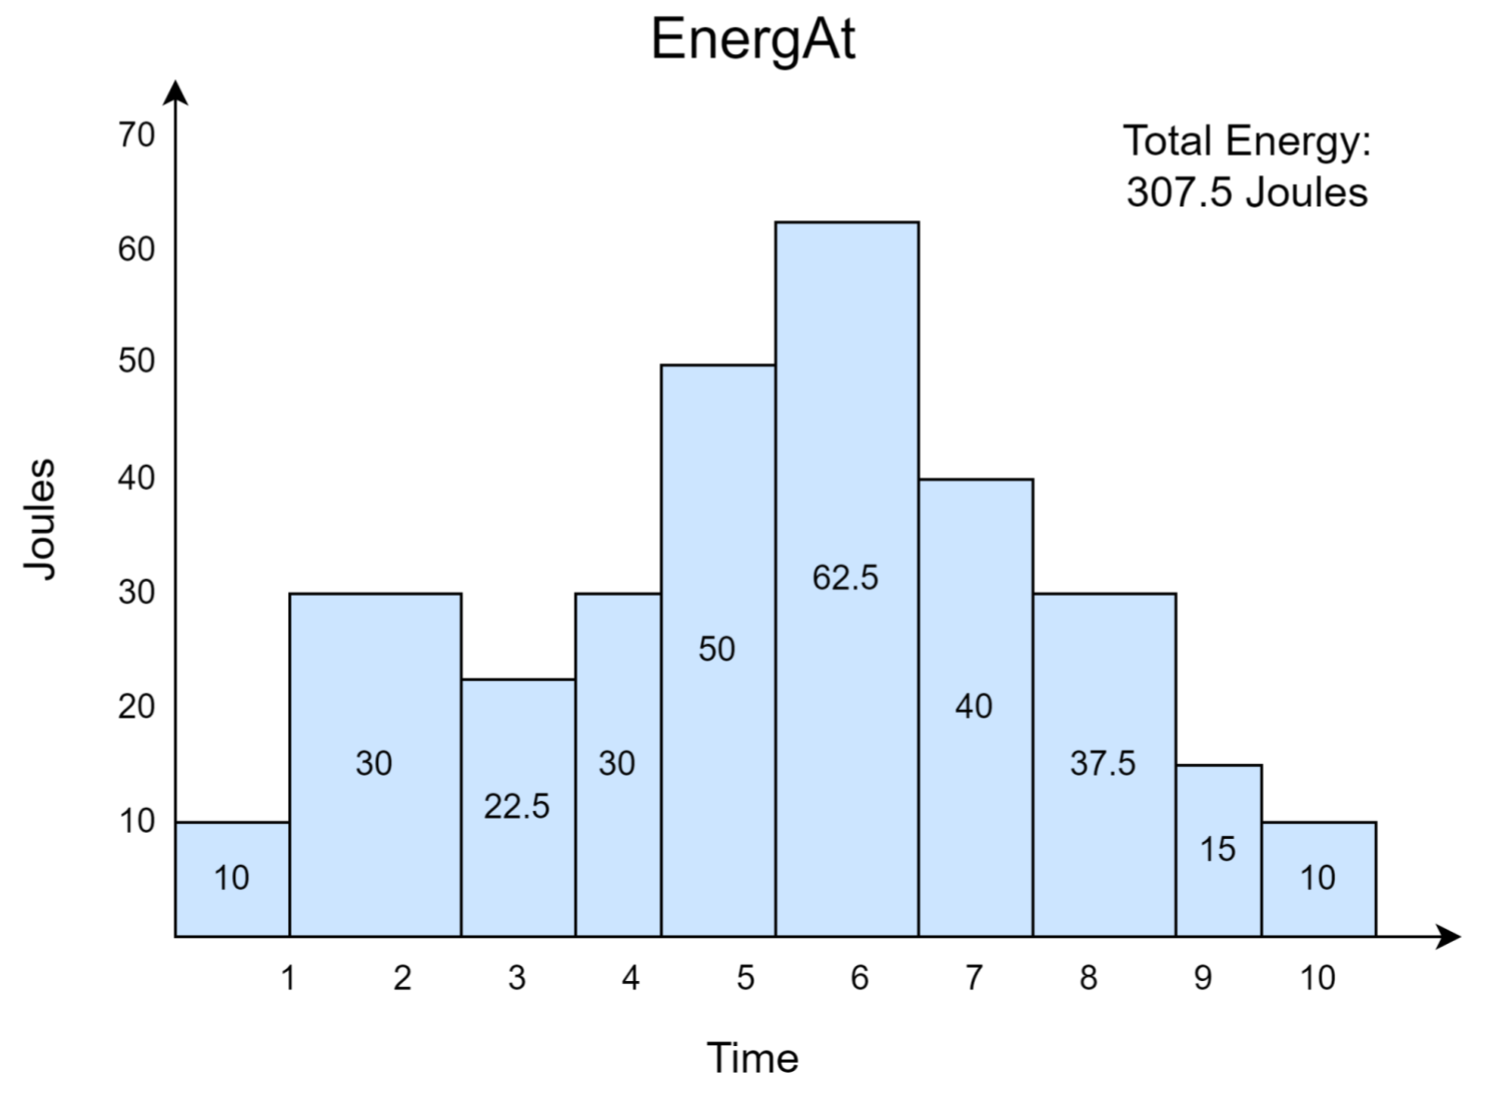
\includegraphics[width=\textwidth]{imgs/EnergAt_Energy.png}
         \caption{}
         \label{fig:a}
   \end{subfigure}
   \hfill
   \begin{subfigure}[b]{0.24\textwidth} % Adjusted width
         \centering
         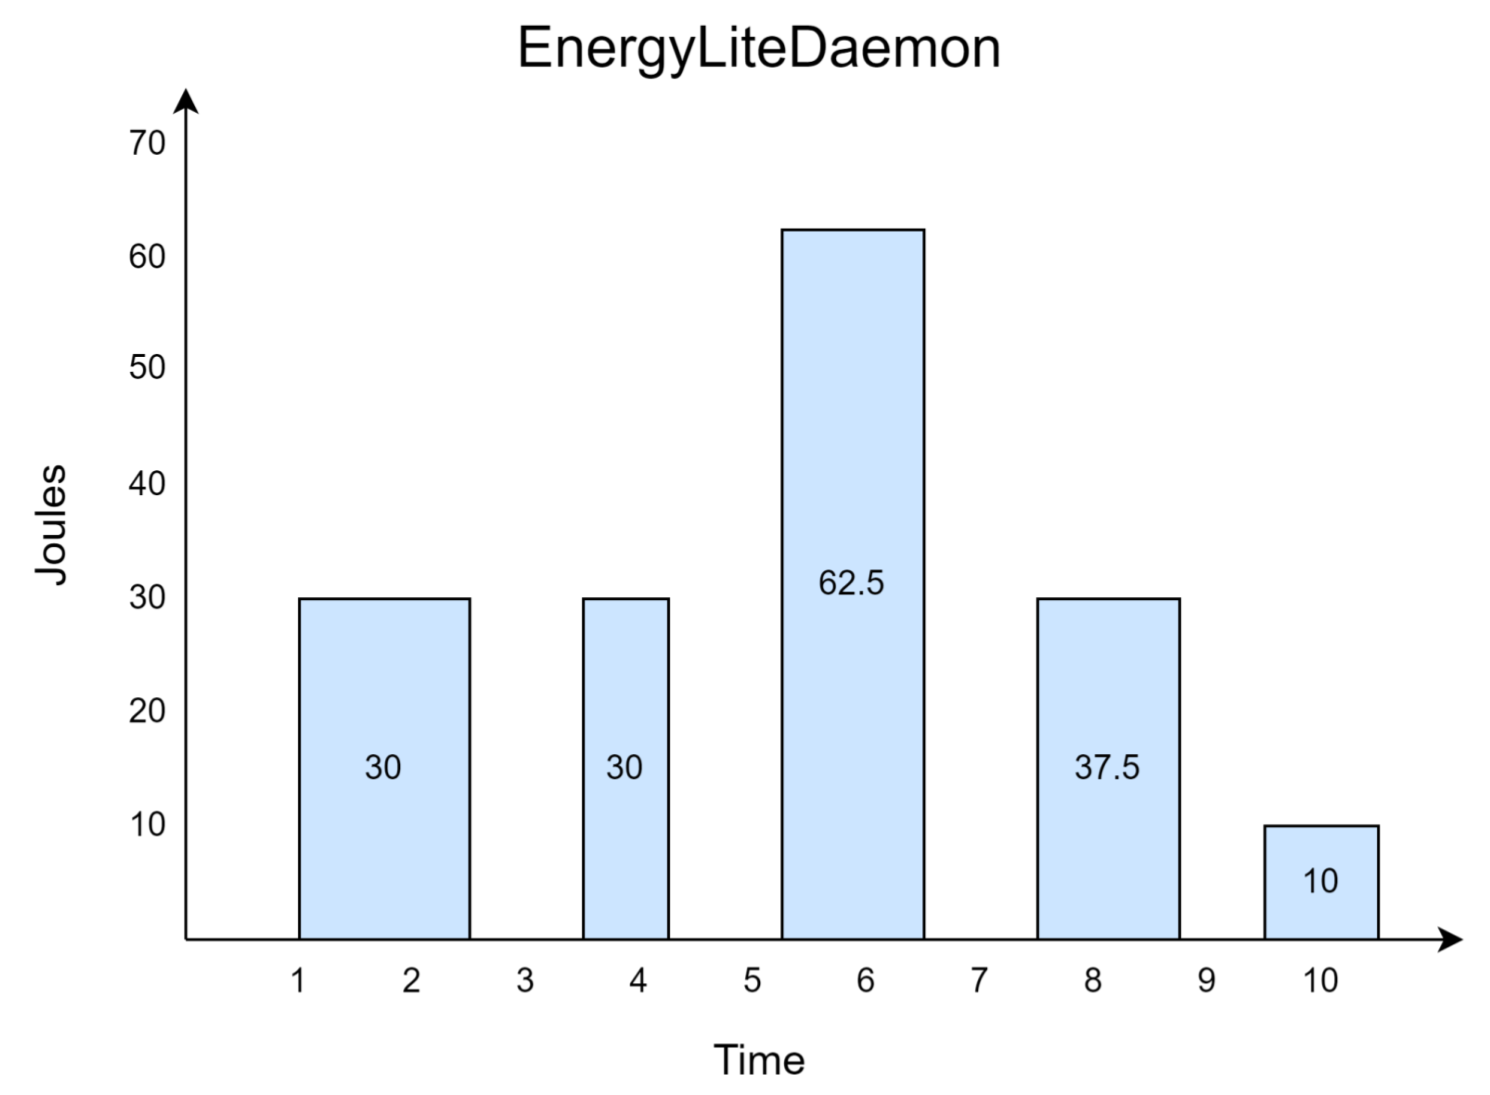
\includegraphics[width=\textwidth]{imgs/EnergyLiteDaemon_Energy_1.png}
         \caption{}
         \label{fig:b}
   \end{subfigure}
   \hfill
   \begin{subfigure}[b]{0.24\textwidth} % Adjusted width
         \centering
         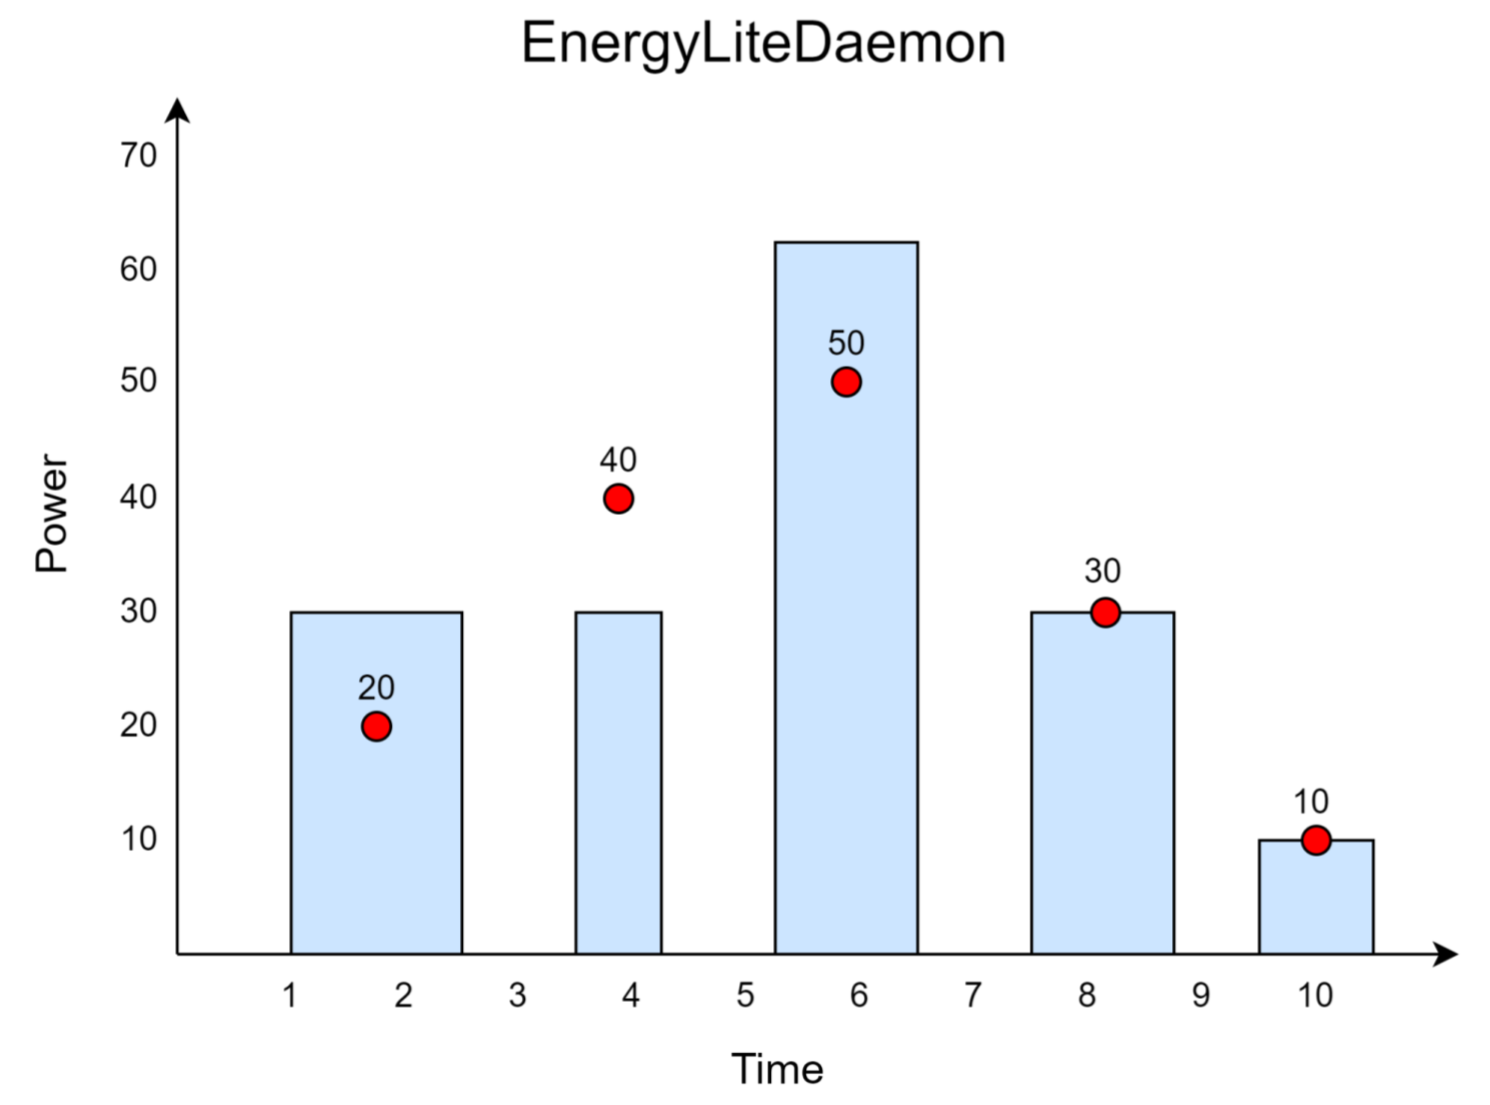
\includegraphics[width=\textwidth]{imgs/EnergyLiteDaemon_Energy_2.png}
         \caption{}
         \label{fig:c}
   \end{subfigure}
   \hfill
   \begin{subfigure}[b]{0.24\textwidth} % Adjusted width
         \centering
         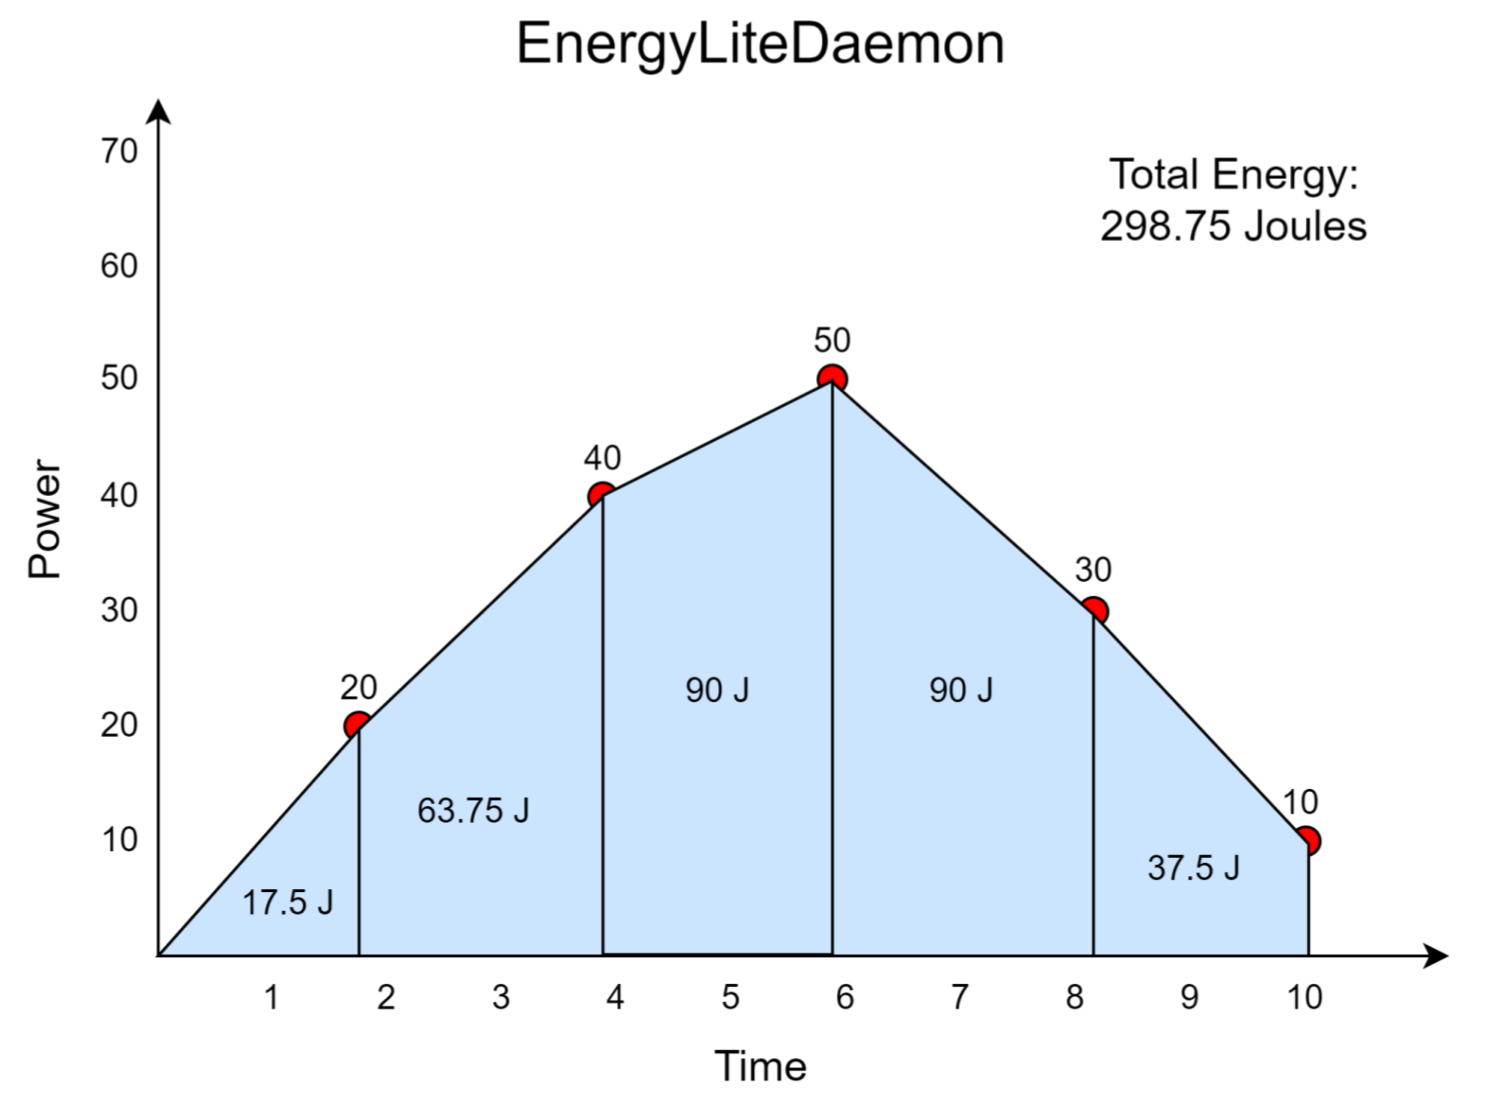
\includegraphics[width=\textwidth]{imgs/EnergyLiteDaemon_Energy_3.png}
         \caption{}
         \label{fig:d}
   \end{subfigure}
   
   \caption{Toy example of energy measurement of a container using EnergAt and EnergyLiteDaemon. (a) EnergAt energy readings. (b) EnergyLiteDaemon energy readings. (c) EnergyLiteDaemon power calculation (red dots). (d) EnergyLiteDaemon energy interpolation using trapezoidal integration.}
   \label{fig:energy_toy_example}
\end{figure*}

\subsection{Energy Variation with vCPU and Frequency Allocation}
\label{appendix:energy_variation_vcpu_frequency}
The energy usage, duration, and CPU usage for Float Matrix Multiplication, Image Processing, and Encryption as a function of vCPU allocation are shown in Figure \ref{fig:cpu_stats}. 

The energy usage and duration for Float Matrix Multiplication, Image Processing, and Encryption as a function of vCPU frequency are shown in Figure \ref{fig:freq_stats}. 
\begin{figure*}[ht]
   \centering
   % First row of plots
   \textbf{Float Matrix Multiplication}\par\medskip
   \begin{subfigure}[b]{0.3\textwidth}
     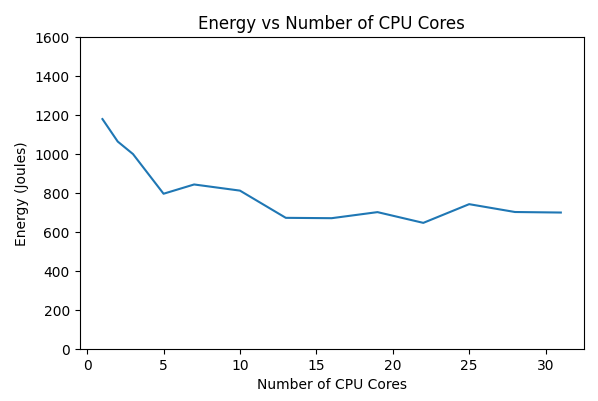
\includegraphics[width=\textwidth]{imgs/study_1_results/var_cpu/floatmatmul/CPU_Energy.png}
     \caption{}
     \label{fig:plot1}
   \end{subfigure}
   \hfill
   \begin{subfigure}[b]{0.3\textwidth}
      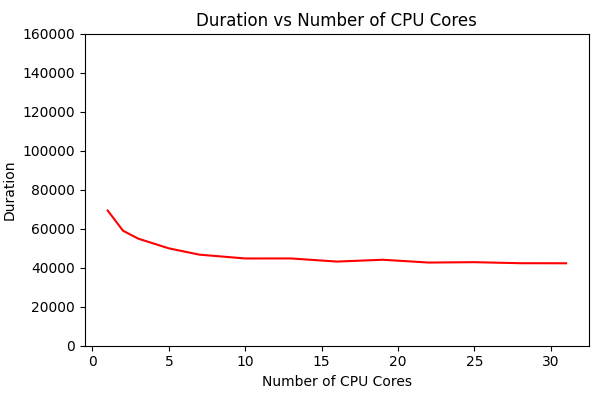
\includegraphics[width=\textwidth]{imgs/study_1_results/var_cpu/floatmatmul/CPU_Duration.png}
     \caption{}
     \label{fig:plot2}
   \end{subfigure}
   \hfill
   \begin{subfigure}[b]{0.3\textwidth}
      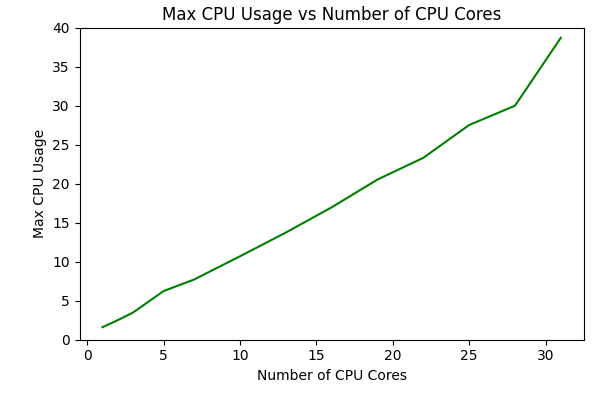
\includegraphics[width=\textwidth]{imgs/study_1_results/var_cpu/floatmatmul/CPU_CPUUsage.png}
     \caption{}
     \label{fig:plot3}
   \end{subfigure}
   % \caption*{Float Matrix Multiplication}
   
   % Second row of plots
   \textbf{Image Process}\par\medskip
   \begin{subfigure}[b]{0.3\textwidth}
      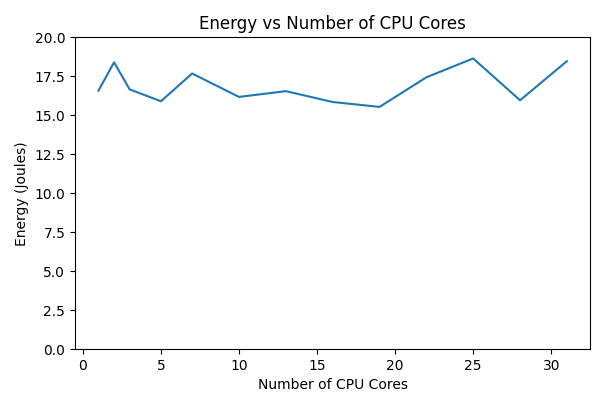
\includegraphics[width=\textwidth]{imgs/study_1_results/var_cpu/imageprocess/CPU_Energy.png}
     \caption{}
     \label{fig:plot4}
   \end{subfigure}
   \hfill
   \begin{subfigure}[b]{0.3\textwidth}
      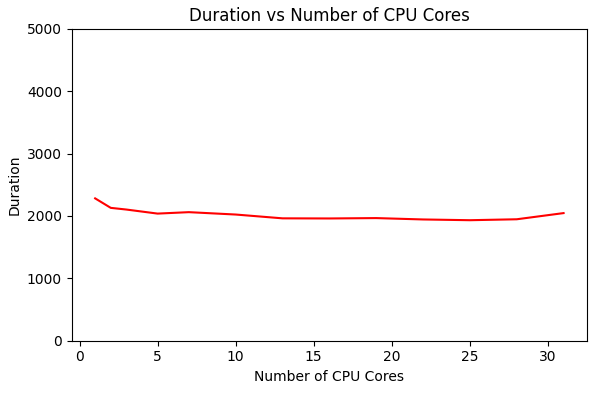
\includegraphics[width=\textwidth]{imgs/study_1_results/var_cpu/imageprocess/CPU_Duration.png}
     \caption{}
     \label{fig:plot5}
   \end{subfigure}
   \hfill
   \begin{subfigure}[b]{0.3\textwidth}
      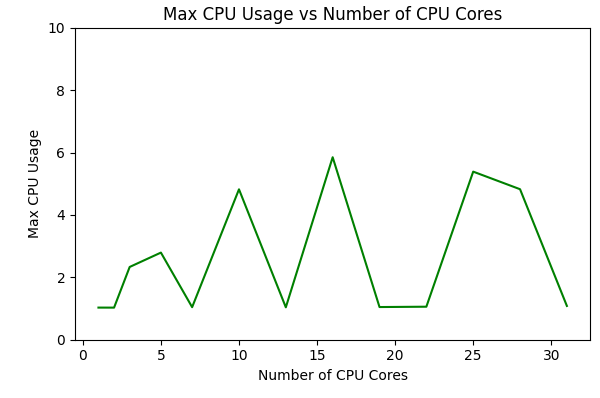
\includegraphics[width=\textwidth]{imgs/study_1_results/var_cpu/imageprocess/CPU_CPUUsage.png}
     \caption{}
     \label{fig:plot6}
   \end{subfigure}
   % \caption*{Image Process}
   
   % Third row of plots
   \textbf{Encryption}\par\medskip
   \begin{subfigure}[b]{0.3\textwidth}
      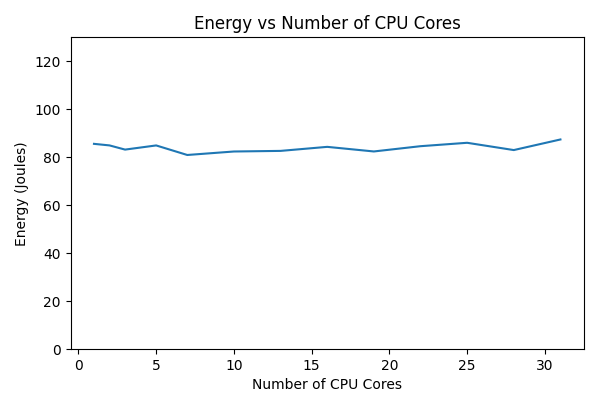
\includegraphics[width=\textwidth]{imgs/study_1_results/var_cpu/encryption/CPU_Energy.png}
     \caption{}
     \label{fig:plot7}
   \end{subfigure}
   \hfill
   \begin{subfigure}[b]{0.3\textwidth}
      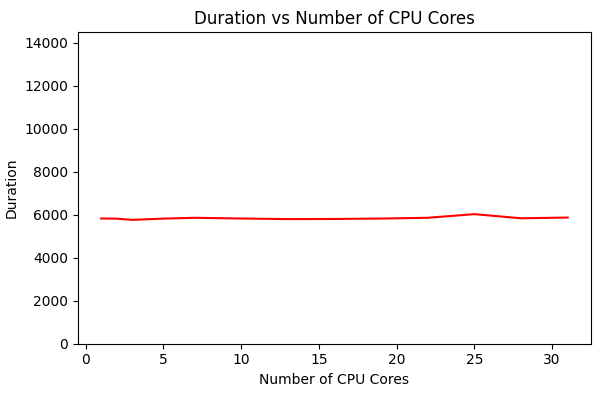
\includegraphics[width=\textwidth]{imgs/study_1_results/var_cpu/encryption/CPU_Duration.png}
     \caption{}
     \label{fig:plot8}
   \end{subfigure}
   \hfill
   \begin{subfigure}[b]{0.3\textwidth}
      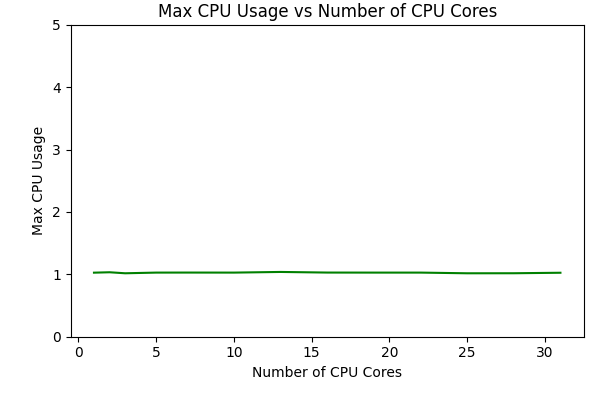
\includegraphics[width=\textwidth]{imgs/study_1_results/var_cpu/encryption/CPU_CPUUsage.png}
     \caption{}
     \label{fig:plot9}
   \end{subfigure}
   % \caption*{Encryption}
   
   \caption{Energy Usage (a), Duration (b), and CPU Usage (c) for Float Matrix Multiplication, Image Processing, and Encryption as a function of vCPU allocation. Frequency was fixed at 2.4 GHz.}
   \label{fig:cpu_stats}
 \end{figure*}
 

 \begin{figure*}[ht]
   \centering
   % First row of plots
   \textbf{Float Matrix Multiplication}\par\medskip
   \begin{subfigure}[b]{0.45\textwidth}
     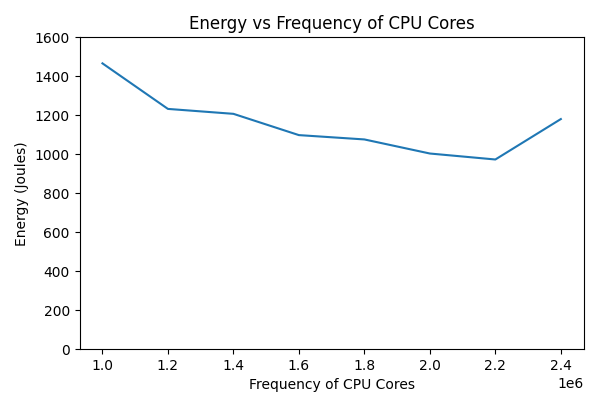
\includegraphics[width=\textwidth]{imgs/study_1_results/var_freq/floatmatmul/Freq_Energy.png}
     \caption{}
     \label{fig:plot10}
   \end{subfigure}
   \hfill
   \begin{subfigure}[b]{0.45\textwidth}
      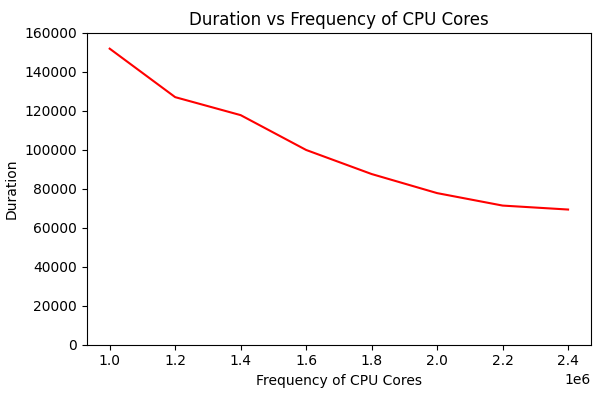
\includegraphics[width=\textwidth]{imgs/study_1_results/var_freq/floatmatmul/Freq_Duration.png}
     \caption{}
     \label{fig:plot11}
   \end{subfigure}
   % \caption*{Float Matrix Multiplication}
   
   % Second row of plots
   \textbf{Image Process}\par\medskip
   \begin{subfigure}[b]{0.45\textwidth}
      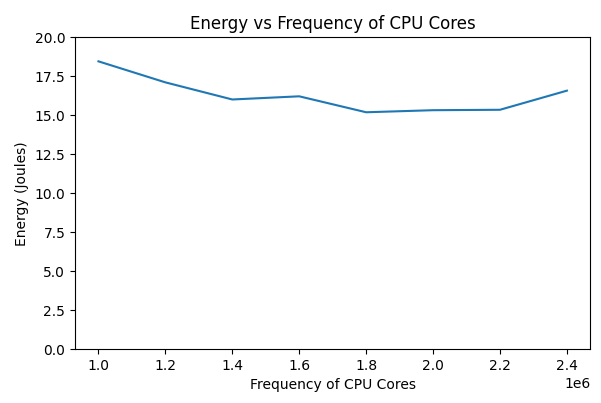
\includegraphics[width=\textwidth]{imgs/study_1_results/var_freq/imageprocess/Freq_Energy.png}
     \caption{}
     \label{fig:plot12}
   \end{subfigure}
   \hfill
   \begin{subfigure}[b]{0.45\textwidth}
      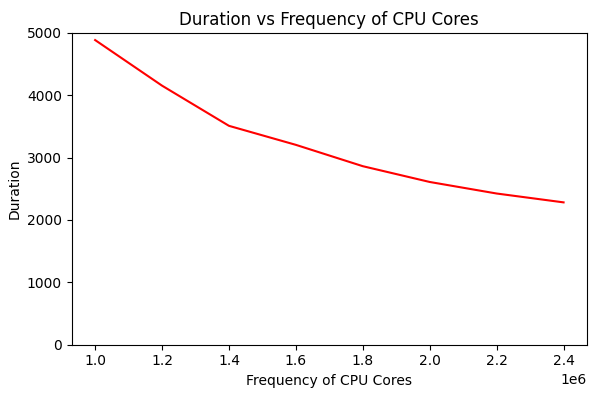
\includegraphics[width=\textwidth]{imgs/study_1_results/var_freq/imageprocess/Freq_Duration.png}
     \caption{}
     \label{fig:plot13}
   \end{subfigure}
   % \caption*{Image Process}
   
   % Third row of plots
   \textbf{Encryption}\par\medskip
   \begin{subfigure}[b]{0.45\textwidth}
      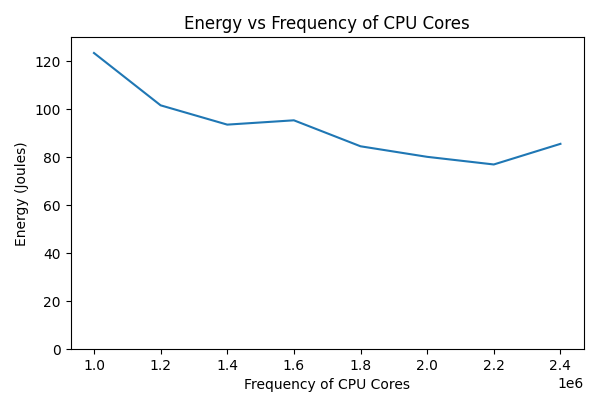
\includegraphics[width=\textwidth]{imgs/study_1_results/var_freq/encryption/Freq_Energy.png}
     \caption{}
     \label{fig:plot14}
   \end{subfigure}
   \hfill
   \begin{subfigure}[b]{0.45\textwidth}
      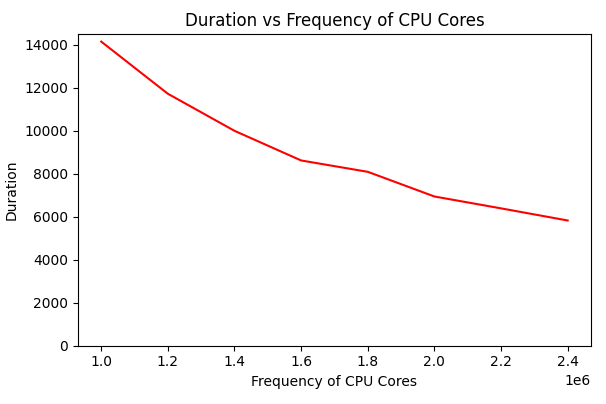
\includegraphics[width=\textwidth]{imgs/study_1_results/var_freq/encryption/Freq_Duration.png}
     \caption{}
     \label{fig:plot15}
   \end{subfigure}
   % \caption*{Encryption}
   
   \caption{Energy Usage (a), Duration (b), and CPU Usage (c) for Float Matrix Multiplication, Image Processing, and Encryption as a function of vCPU frequency. vCPU allocation was fixed at 1.}
   \label{fig:freq_stats}
 \end{figure*}
 
 \subsection{Energy Variation for Different Stages of a Serverless Function Invocation}
 \label{appendix:energy_variation_vcpu_memory}
 We can see here the energy consumption of the container spin-up, idle time, and container spin-down for different image sizes in Figure \ref{fig:energy_stages}. 

 \begin{figure*}[ht]
   \centering
   % First row of plots
   \textbf{Spin Up Stage}\par\medskip
   \begin{subfigure}[b]{0.3\textwidth}
     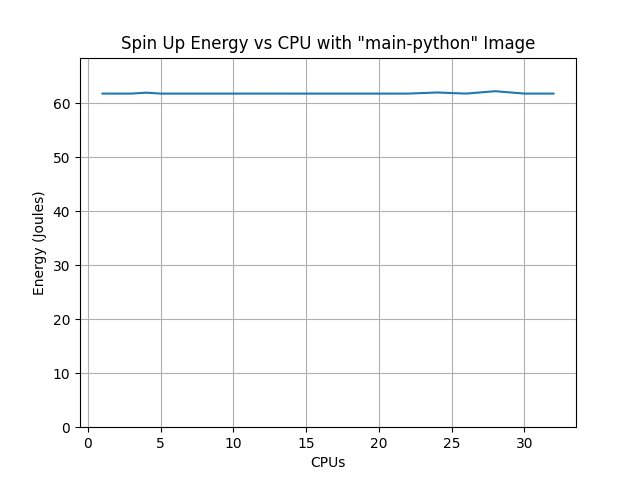
\includegraphics[width=\textwidth]{imgs/container_study/spin_up_vs_cpu.png}
     \caption{}
     \label{fig:spin_up_cpu}
   \end{subfigure}
   \hfill
   \begin{subfigure}[b]{0.3\textwidth}
      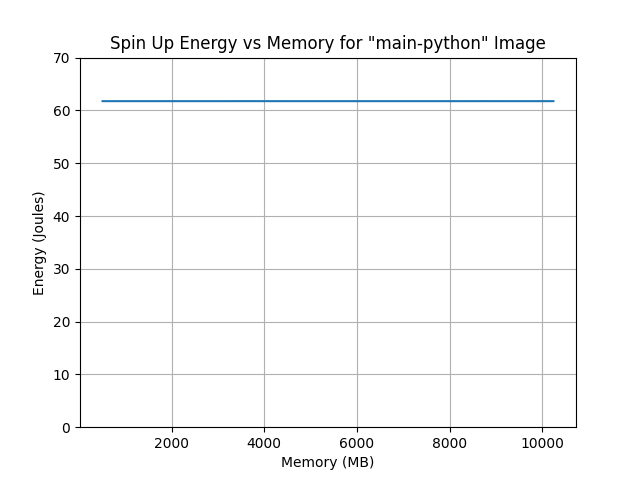
\includegraphics[width=\textwidth]{imgs/container_study/spin_up_vs_mem.png}
     \caption{}
     \label{fig:spin_up_mem}
   \end{subfigure}
   \hfill
   \begin{subfigure}[b]{0.3\textwidth}
      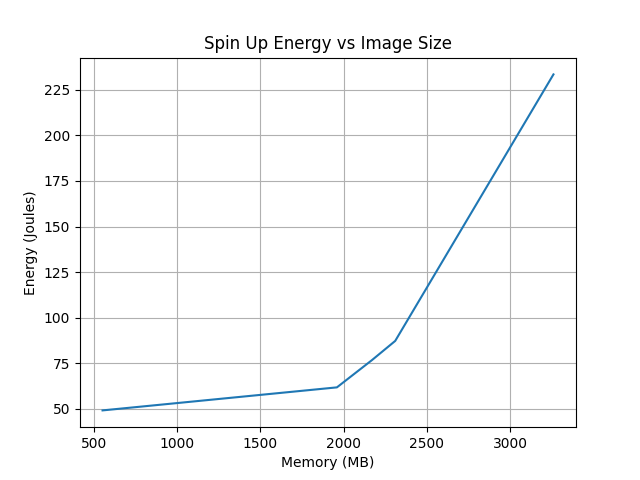
\includegraphics[width=\textwidth]{imgs/container_study/spin_up_vs_image.png}
     \caption{}
     \label{fig:spin_up_img}
   \end{subfigure}
   % \caption*{Float Matrix Multiplication}
   
   % Second row of plots
   \textbf{Spin Down Stage}\par\medskip
   \begin{subfigure}[b]{0.3\textwidth}
      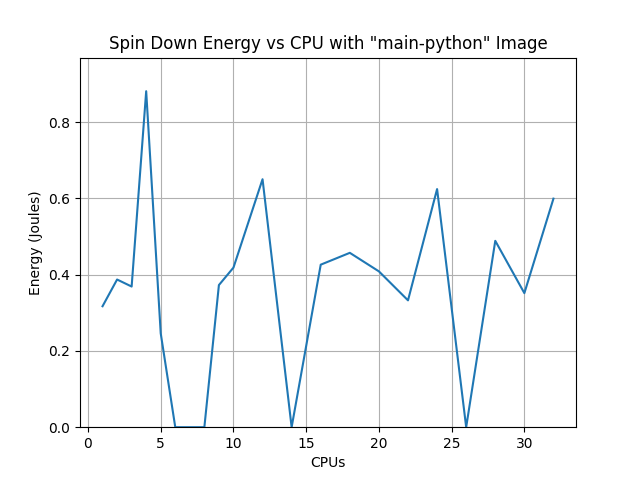
\includegraphics[width=\textwidth]{imgs/container_study/spin_down_vs_cpu.png}
     \caption{}
     \label{fig:spin_down_cpu}
   \end{subfigure}
   \hfill
   \begin{subfigure}[b]{0.3\textwidth}
      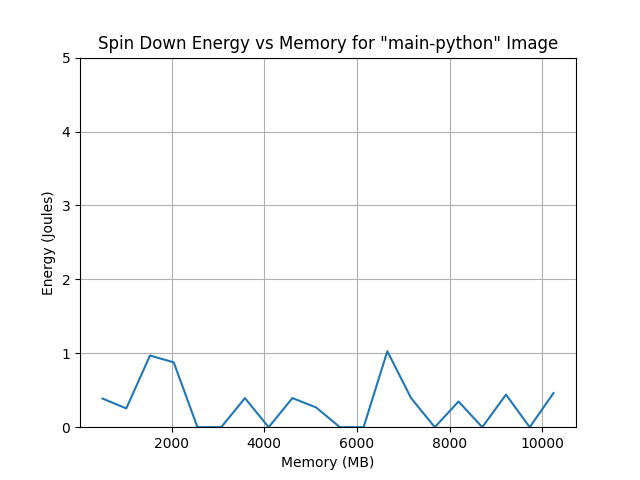
\includegraphics[width=\textwidth]{imgs/container_study/spin_down_vs_mem.png}
     \caption{}
     \label{fig:spin_down_mem}
   \end{subfigure}
   \hfill
   \begin{subfigure}[b]{0.3\textwidth}
      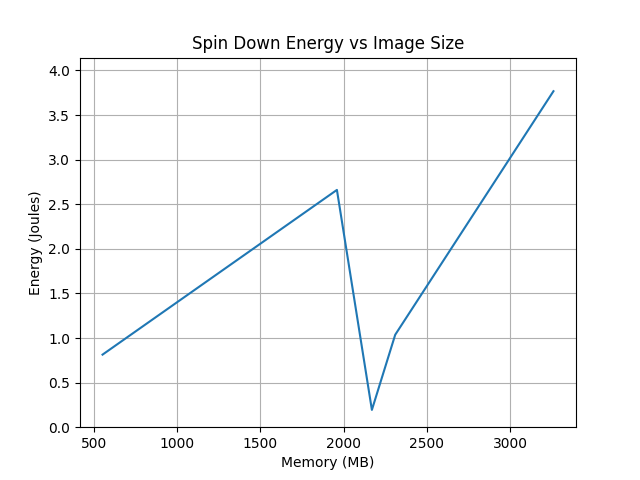
\includegraphics[width=\textwidth]{imgs/container_study/spin_down_vs_image.png}
     \caption{}
     \label{fig:spin_down_img}
   \end{subfigure}
   % \caption*{Image Process}
   
   % Third row of plots
   \textbf{Idle Stage}\par\medskip
   \begin{subfigure}[b]{0.3\textwidth}
      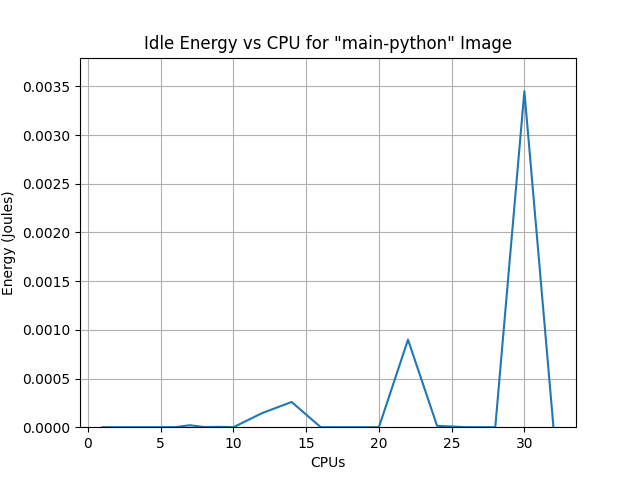
\includegraphics[width=\textwidth]{imgs/container_study/idle_vs_cpu.png}
     \caption{}
     \label{fig:idle_cpu}
   \end{subfigure}
   \hfill
   \begin{subfigure}[b]{0.3\textwidth}
      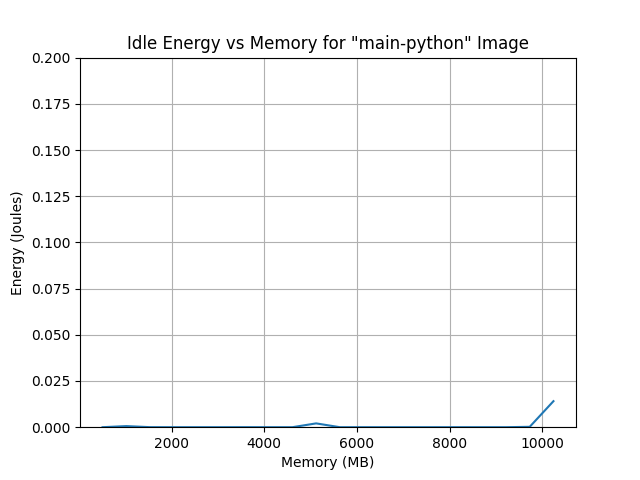
\includegraphics[width=\textwidth]{imgs/container_study/idle_vs_mem.png}
     \caption{}
     \label{fig:idle_mem}
   \end{subfigure}
   \hfill
   \begin{subfigure}[b]{0.3\textwidth}
      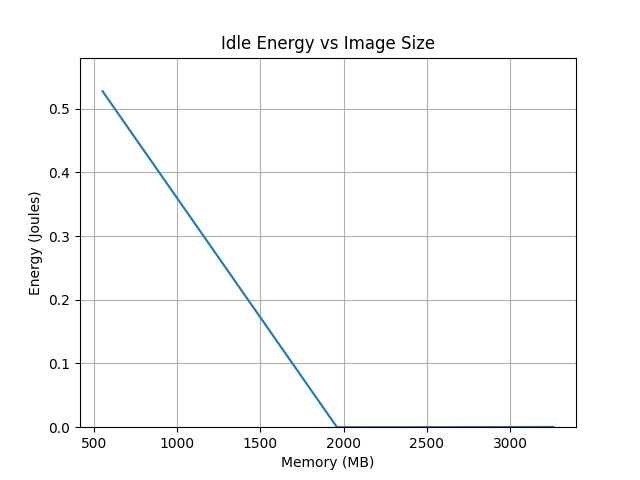
\includegraphics[width=\textwidth]{imgs/container_study/idle_vs_img.png}
     \caption{}
     \label{fig:idle_img}
   \end{subfigure}
   % \caption*{Encryption}
   
   \caption{Energy Usage vs CPU (a, d, g), Memory (b, e, h), and Image Size (c, f, i) for the Spin Up, Spin Down, and Idle stages of a serverless function invocation.}
   \label{fig:energy_stages}
 \end{figure*}

\end{document}
